% This file was created by matplotlib2tikz v0.6.13.
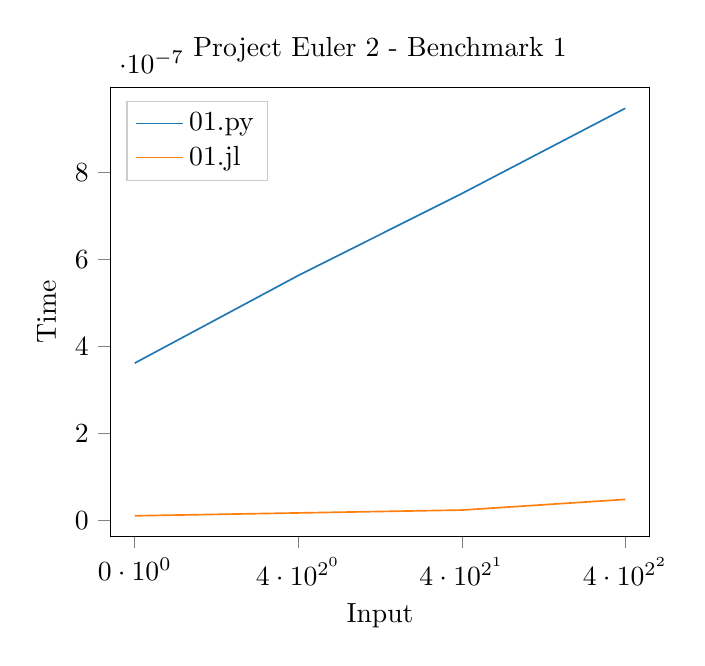
\begin{tikzpicture}

\definecolor{color1}{rgb}{1,0.498039215686275,0.0549019607843137}
\definecolor{color0}{rgb}{0.12156862745098,0.466666666666667,0.705882352941177}

\begin{axis}[
title={Project Euler 2 - Benchmark  1 },
xlabel={Input},
ylabel={Time},
xmin=-0.15, xmax=3.15,
ymin=-3.57788179202607e-08, ymax=9.95227048197346e-07,
xtick={0,1,2,3},
xticklabels={$0 \cdot 10^{0}$   ,$4 \cdot 10^{2^0}$ ,$4 \cdot 10^{2^1}$ ,$4 \cdot 10^{2^2}$ },
tick align=outside,
tick pos=left,
x grid style={lightgray!92.026143790849673!black},
y grid style={lightgray!92.026143790849673!black},
legend entries={{01.py},{01.jl}},
legend cell align={left},
legend style={at={(0.03,0.97)}, anchor=north west, draw=white!80.0!black}
]
\addlegendimage{no markers, color0}
\addlegendimage{no markers, color1}
\addplot [semithick, color0]
table {%
0 3.62247625987e-07
1 5.63732783e-07
2 7.52146244049e-07
3 9.48363145192e-07
};
\addplot [semithick, color1]
table {%
0 1.10850850850851e-08
1 1.76830491474423e-08
2 2.42771084337349e-08
3 4.87338709677419e-08
};
\end{axis}

\end{tikzpicture}